%!Mode:: "TeX:UTF-8"
%!TEX program = xelatex
%!TEX TS-program = xelatex
%!TEX encoding = UTF-8 Unicode
%
% Author: Rickjin (ZhihuiJin@gmail.com)
% Author: Leijun 

\chapter{从Google 说起}

\section{字母的江湖地位}
对各类事物论资排辈理出个江湖地位是人们闲时的重要消遣,世界大学的排名、科学家的
贡献、金庸小说中各位大侠的战斗力,无不是互联网网友们唾沫横飞争个面红耳赤的重要
话题。 今天我们想争论的一个问题是:在文字的世界里,哪个字母的江湖地位排名第
一?如果限制在英语的26个字母中, 这个问题也许相对容易回答,很多人应该会选择字母
$e$。即便在全世界的文字中来投票,预计字母$e$占据头把交椅的可能性也最高,毕竟英
语是准国际语言。 学过英语的读者利用自己的直觉也不难感知到字母 $e$ 是英语中使用
频率最高字母。而这种主观感觉和实际的统计结果是非常符合的,下表列出了26个英语字
母的使用频率( 这个表的来源最好说明一下)。

\begin{table}[htbp]
\centering
\caption{英文字母使用频率(百分比)}
\begin{tabular}{|l|}
\hline
A 8.19 B 1.47 C 3.83 D 3.91 E 12.25      \\ \hline
F 2.26 G 1.71 H 4.57 I 7.10 J 0.14       \\ \hline
K 0.41 L 3.77 M 3.34 N 7.06 O 7.26       \\ \hline
P 2.89 Q 0.09 R 6.85 S 6.36 T 9.41       \\ \hline
U 2.58 V 1.09 W 1.59 X 0.21Y 1.58 Z 0.08 \\ \hline
\end{tabular}
\centering
\end{table}

顺着这个思路我们抛出一个问题:如果限制在数学王国中,哪个字母能夺得桂冠呢? 虑到
希腊字母在数学世界中的霸主地位,$\pi$ 预计能够傲视其他一切数学字母。但是如果把
问题稍微改变一点:举办一场数学王国中的字母选美比赛,数学王国中的字母都可以报名
参加,哪位将夺得桂冠?这个问题可能会变得很有争议,而字母 $e$ 绝对是一个实力雄厚
的竞争者。我们的《传奇e事》系列就是要来讲讲和字母 $e$ 相关的数学故事,相信读者
们读完很多和$e$ 相关的故事之后,会更加认同 $e$ 是在数学王国中是是有绝对的竞选实
力的。 

\section{巨头的数学基因}
$e$ 在数学王国中自然是一个有故事的字母,然而我们不用着急了解它的历史, 先把时间
拉到现代,看看现代人是如何看待$e$的。 我们的故事先从著名的互联网巨头 Google 说
起。

Google 是一个大家都很熟悉的公司,她创造了世界上最庞大的搜索引擎,以免费的形式为
全世界人民提供了大量的互联网产品和服务。如果把互联网比作江湖,那么Google、
Amazon、 Facebook、Yahoo 这些公司都是来自美国的江湖大侠。同样地 BAT(百度、阿里
和腾讯)这三家公司是来自中国的大侠。那谁会是这个互联网江湖的武林盟主呢?绝大多
数人会推举 Google 作为互联网江湖的武林盟主。天下武功出少林,互联网的一流技术大
都源自 Google。Google 成为了计算机工程师(俗称码农)朝圣的地方,很多计算机系的
毕业生在毕业时都希望能进入 Google,只要在 Google 学了一招半式,脑门上就会有技术
的光环,出来以后在互联网江湖里就会变得受人尊重。

% ref http://graphics.stanford.edu/~dk/google_name_origin.html
% https://www.google.com.hk/intl/zh-CN/about/company/
然而很多人也许并不知道, Google 同时是一家非常具有数学基因的公司,她其实是一个
数学的超级大粉丝,在很多的重要活动和事件中Google 都表达出对数学的热爱。首先我们
来看看 Google 这个公司的命名,名字本身就具有浓厚的数学味: Google 这个词其实是
源自数学名词 Googol,这个词代表了一个天文数字,原始的含义表示1后面跟着100个零(
即 10 的100次方)。令人吃惊的是,Googol这个词历史上可是由一个9岁大的小屁孩创造
的,他是美国数学家Edward Kasner 的外甥 Milton Sirotta, 而这个词通过 Kasner 和
James Newman 合著的《数学和想象》( Mathematics and the Imagination)一书而广为
流传。

既然最早的词形是 Googol, 为何最终公司名字会演变成 Google 了呢?这背后有一些有意
思的故事。 Google 的创始人 Larry Page 和 Sergey Brin 梦想整合互联网上海量信息,
在 1997年的时候他们考虑为公司注册一个和海量数据相关的域名。两位创始人和几位大四
本科生一起头脑风暴,在本科生 Sean Anderson 建议下大家聚焦到了 Googol 这个数学名
词:由于 Googol 代表了 $10^100$, 所以毫无疑问这是一个好名字。 于是Sean 尝试在域
名服务上进行检索注册,结果Sean 第一次输入的时候把域名阴错阳差的敲成了
"google.com",同时发现这个域名可用。而实际上纠正拼写后却遗憾的发现 "googol.com"
已经是他人的禳中之物了。 这可如何是好? 真是无巧不成书,Larry 却很喜欢这个拼写
错误的的版本 "google", 于是他们迅速敲定为公司注册了域名 "google.com" 。 


第二个反映 Google 数学基因的例子就是Google 涂鸦(Google Doodle),Google 创造了一
种艺术形式:在一些重要的日子里把公司网站门面上的 Logo 进行重新设计,通过各种艺
术形式把 Google 这个单词和重要的日子关联起来,借以纪念相关的人物或事件。而在和
数学相关的重要节日中, Google 就会推出一些别出心裁的数学涂鸦。下图种列举了一些
比较有名的数学涂鸦,你能猜出来每一个涂鸦都是在纪念哪些重要的数学事件或人物吗?

\footnote{
从左到右,从上到下分别是:
2014年3月14日\href{http://www.google.com/doodles/pi-day?hl=zh-CN}{圆周率日},
2010年10月11日\href{http://www.google.com/doodles/cahit-arfs-100th-birthday?hl=zh-CN}{贾希特·阿尔夫诞辰100周年} ,
2004年2月2日\href{http://www.google.com/doodles/gaston-julias-111th-birthday?hl=zh-CN}{加斯顿·朱丽亚诞辰111周年},
2009年4月20日\href{http://www.google.com/doodles/zu-chongzhis-birthday?hl=zh-CN}{祖冲之诞辰纪念日},
2011年11月12日\href{http://www.google.com/doodles/hua-luogengs-101st-birthday?hl=zh-CN}{华罗庚诞辰101周年},
2015年3月23日\href{http://www.google.com/doodles/emmy-noethers-133rd-birthday?hl=zh-CN}{埃米·诺特诞辰 133 周年},
2011年8月17日\href{http://www.google.com/doodles/pierre-de-fermats-410th-birthday?hl=zh-CN}{皮埃尔·德·费玛诞辰410周年},
2013年4月15日\href{http://www.google.com/doodles/leonhard-eulers-306th-birthday?hl=zh-CN}{莱昂哈德·欧拉诞辰306周年},
2012年12月22日\href{http://www.google.com/doodles/srinivasa-ramanujans-125th-birthday?hl=zh-CN}{斯里尼瓦瑟·拉马努金诞辰125周年},
2014年8月4日\href{http://www.google.com/doodles/john-venns-180th-birthday?hl=zh-CN}{约翰·维恩诞辰180周年},
2012年6月23日\href{http://www.google.com/doodles/alan-turings-100th-birthday?hl=zh-CN}{阿兰·图灵诞辰100周年}。
}

\begin{figure}[htbp]
\centering
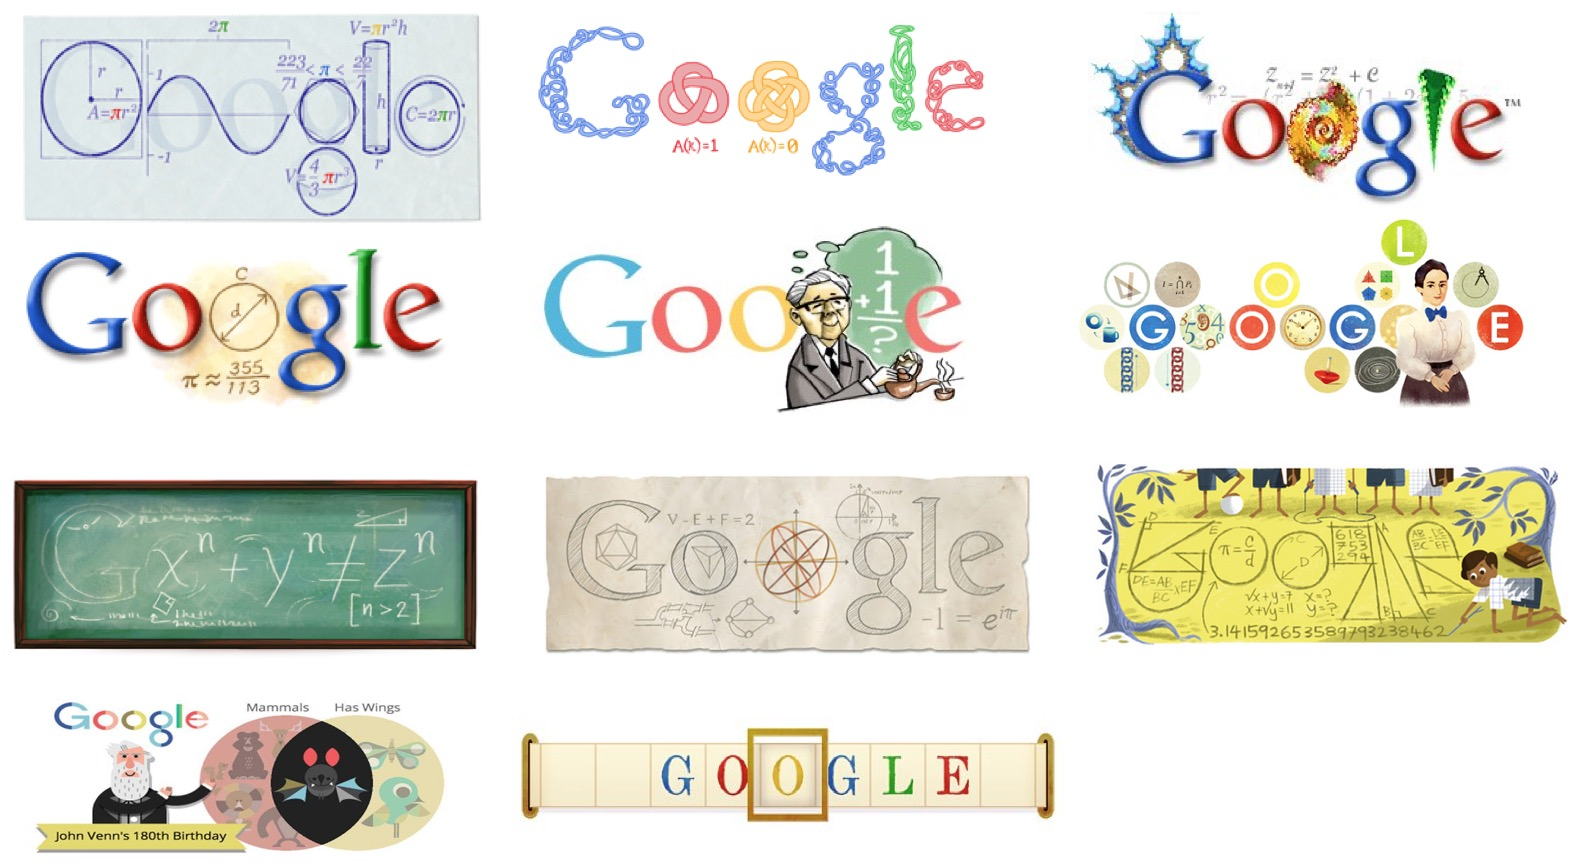
\includegraphics[scale=0.5]{google/doodle.png}
\caption{Google 数学涂鸦}
\centering
\end{figure}

% Google一个多月前回购股票金额$5,099,019,513.59,是26的平方根,因为Alphabet里有26个字母。

\section{$e$之恋}

我们继续 Google 的数学故事。 2014年8月19日Google 在纳斯达克上市,市的时候需要融
资啊,需要融多少钱呢?Google 提交的 IPO S-1 表格上写一个非常有意思的金额:
$2,718,281,828$ 美元。这个数字一给出,华尔街一片哗然,不知道 Google 为什么选择
这样一个奇怪的数字,有零有整,精确到一美元!按照华尔街的惯例,一般公司上市
的时候会选择的融资金额大约会精确到千万、百万美元,几乎没有精确到一美元的。
Google 直接宣布融资 27.1亿美元不就行了,给一个具体到个位数的融资额度真是咄咄怪
事。但是数学粉丝们一看到这个数字,都非常的兴奋,他们对这个数字再熟悉不过了:
$2,718,281,828$ 恰恰是一个著名的数学无理数 $e$ 的前十位。


\begin{figure}[htbp]
\centering
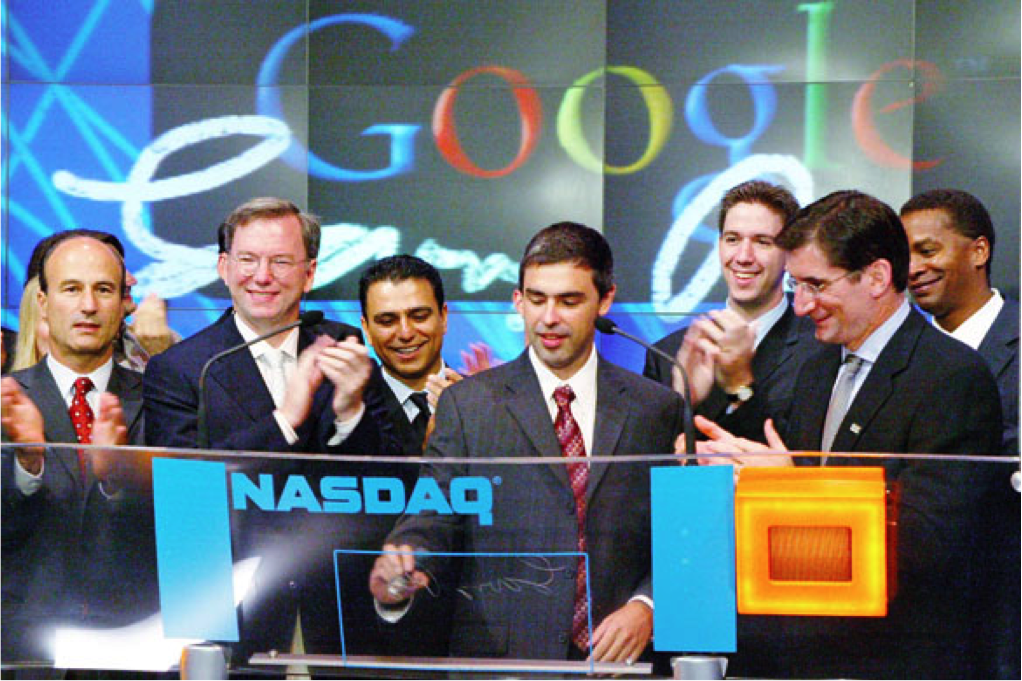
\includegraphics[scale=0.5]{google/ipo.png}
\caption{Google 上市}
\centering
\end{figure}

上市对任何一个公司而言都是极其重要的日子,是一个 Big Day, 类似女孩子长大成人出
嫁,能够上市那是一个公司在市场上成功的标志。 Google 在上市的时候选择无理数 $e$
的前十位来作为融资额度,不单单是表达对无理数 $e$ 的喜爱,应该说这是在致敬无理数
$e$。

\begin{figure}[htbp]
\centering
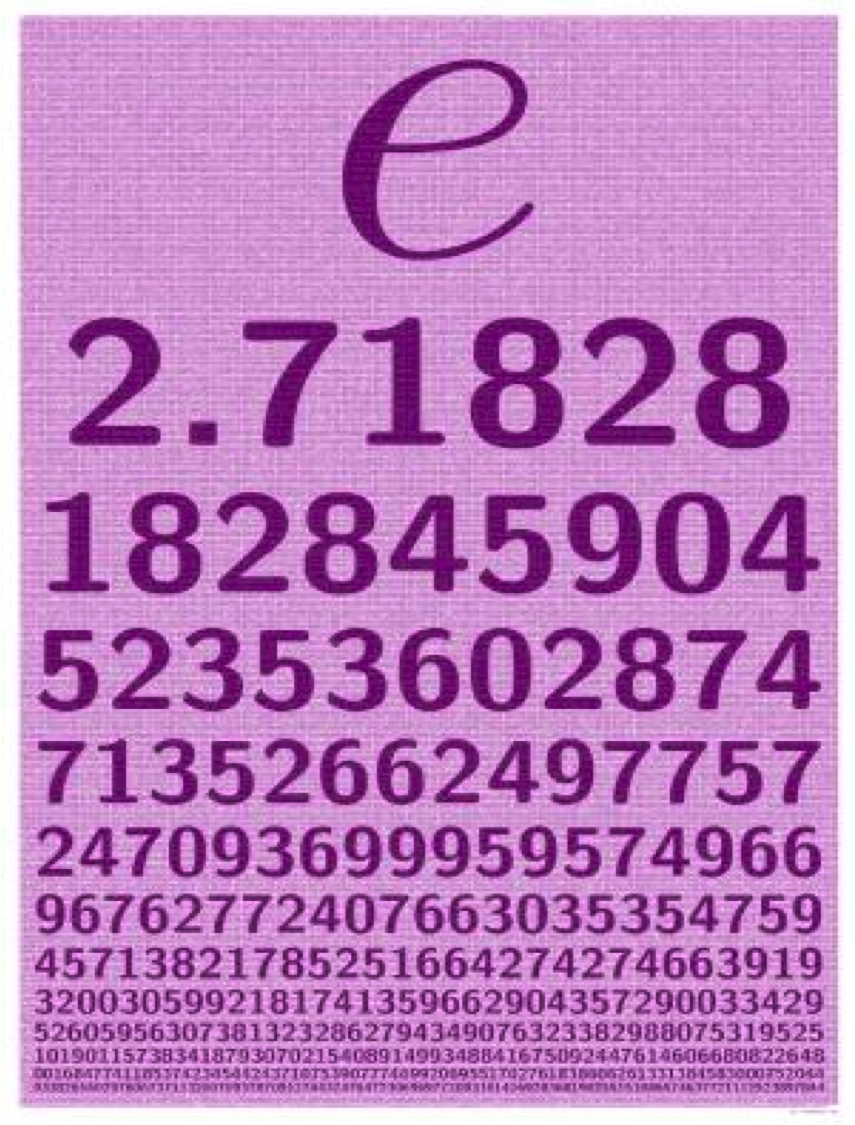
\includegraphics[scale=0.3]{google/e-digits.png}
\caption{无理数 $e$ 的小数展开}
\centering
\end{figure}
大家都知道实数轴王国里面住着有无穷多的无理数公民,但是有三位无理数大侠那是极负
盛名:圆周率 $\pi$、自然常数 $e$ 和 黄金分割比 $\phi$,号称“数学三圣”。
Google 对这三大无理数都钟爱有加,据说 Google 发展历史上曾经有四幢办公楼,而这几
幢办公楼的命名非常奇特: 第二幢办公楼的名称就叫 $e$ 办公楼,第三幢办公楼叫
$\pi$,第四幢办公楼则命名为 $\phi$。

\begin{figure}[htbp]
\centering
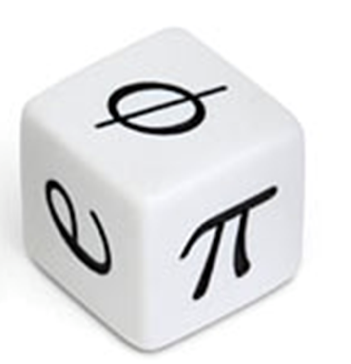
\includegraphics[scale=0.5]{google/dice.png}
\caption{无理数三圣}
\centering
\end{figure}

我们再来讲一个有意思的数学故事。 2004年7月在美国加州硅谷 101公路的旁边立起了一
个巨大的广告牌,这个广告牌特别奇怪,不广告任何商品,上面只有一行字:"$\{$the
first 10-digit prime in consecutive digits of $e$ $\}$.com" ,翻译成中文就是:
"$\{$常数e中出现的第一个10位质数$\}$.com"。很快,相同的广告牌陆续出现在了西雅图
、哥伦比亚、马塞诸塞、华盛顿、奥斯丁、德克萨斯等美国各大州,引起了极大的关注度
。很多人不禁感到奇怪:哪个公司这么有钱,打这么一个令人看不懂的奇怪广告?

\begin{figure}[htbp]
\centering
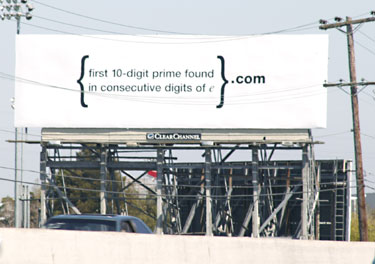
\includegraphics[scale=0.8]{google/billboard.jpg}
\caption{硅谷的广告牌}
\centering
\end{figure}

然而数学粉丝们一看这个广告牌就被吸引了,很明显这是一道数学挑战题。无理数的小数
展开在数学史上算是一个老生常谈了,最有名的莫过于$\pi$ 的小数展开的计算。 历史上
众多数学家呕心沥血的计算$\pi$ 的近似值,留下了许多可歌可泣的数学故事。 而这道题
中显然要求的是计算无理数$e$ 的小数展开。 同时题目中在数字答案后面追加了一个
".com" ,明确暗示了一个网站地址, 而登录这个网站的钥匙就是无理数$e$中出现的第一
个10位质数。

众多数学粉丝们摩拳擦掌,纷纷开始了挑战。要解出这个题目可不简单, 需要编写程序把
无理数$e$ 的小数展开计算到很多位,所以不但要求有丰富的数学知识,而且要求出色的
计算机编程技能。 数学和计算机的爱好者们写完程序,在计算机上最终算出来这个10位质
数是7427466391,他们很兴奋的登录网站 7427466391.com 一看究竟,结果发现网站里面
又冒出了一道新的数学题 ,这道题比广告牌里的数学题还难。数学爱好者们又被这道题所
吸引,继续迎接新的挑战,攻克完这道题之后,接下来又遇到了几道题,这不就是升级打
怪嘛! 面对层层关卡的筛选,最终能够留下的人也就不多了,然而总有一些出色的计算机
和数学爱好者们打了通关最后到达了终点站,最后的页面上显示:欢迎你投递简历到
Google实验室。

大家终于恍然大悟:原来那个奇怪的广告牌是 Google 公司的招聘广告。而在这个招聘流
程中, Google 的工程师们选择了 $e$ 这个无理数作为面试题,充分表达他们对无理数
$e$ 的喜爱。
	
\section{$e$ 是什么}
讲完了 Google 和 $e$ 的故事,最后来看看 $e$ 到底是什么?中学里我们就接触过 $e$
,那时候我们知道 $e$ 约等于 2.718281828,$e$ 是自然对数的底数。
$$ e \approx 2.718281828 $$
$$ ln(x) = log_{e}(x) . $$ 
在高中的时候, 我们会学习到$e$ 的定义是一个极限
$$ e = \lim_{n \to \infty}(1+\frac{1}{n})^n  .$$

上了大学学习微积分、概率论、数学分析以后,我们就会接触到越来越多跟 $e$ 相关的知
识,而我们也会产生很多的疑问: $e$ 到底是一个什么样的数? $e$ 有什么有趣的性质
?$e$ 和我们的日常生活有什么联系?$e$ 有多少年的历史? 历史上数学家是如何发现
$e$ 的?为何以 $e$ 为底的对数称为自然对数? 为什么 $e$ 有那么多名字,同时被称为
自然常数、欧拉常数、纳皮尔常数?为什么 Google 和许多数学人如此喜欢 $e$?

著名的数学科普大师马丁·加德纳(Martin Gardner,1914年10月21日— 2010年05月22日
)发现,三个无理数大侠中,学生们对圆周率 $\pi$ 和黄金分割比 $\phi$都是比较熟悉
的,而对自然常数 $e$ 却是最不熟悉的。你是否熟悉 $e$ 呢?可以简单做一个测试, 下
面是一张由单词组成的字母 $e$ 图片,这个图片里面的每一个单词都跟 $e$ 的某些性质
相关,有多少性质你是熟悉的?如果读者也不熟悉的话,欢迎接下来的时间一起学习关于
$e$ 的传奇故事。
\begin{figure}[htbp]
\centering
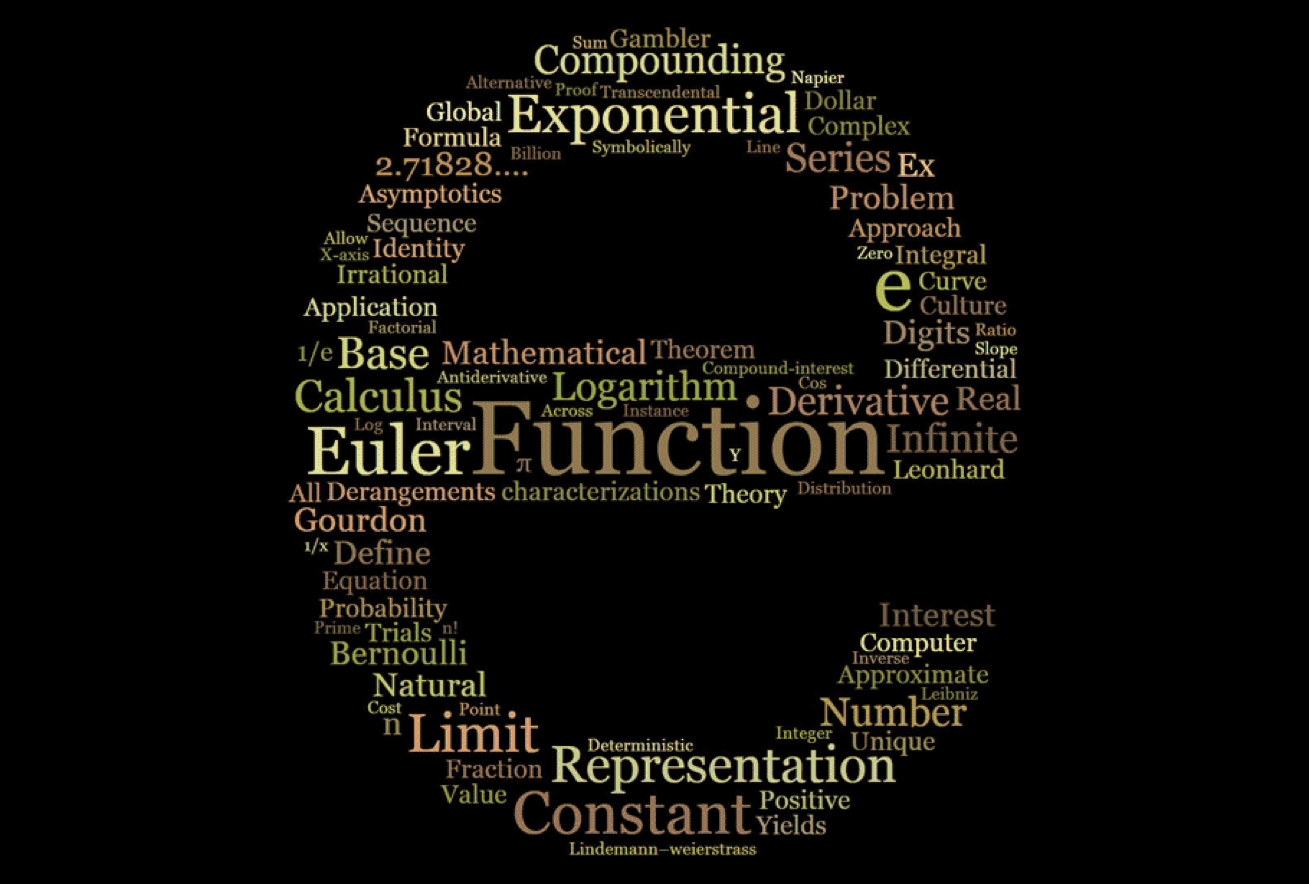
\includegraphics[scale=0.5]{google/eword.png}
\caption{$e$ 单词云}
\centering
\end{figure}


